\documentclass{article}

\usepackage{dirtree}

\usepackage[
  height=9in,      % height of the text block
  width=7.5in,       % width of the text block
  top=78pt,        % distance of the text block from the top of the page
  headheight=48pt, % height for the header block
  headsep=12pt,    % distance from the header block to the text block
  heightrounded,   % ensure an integer number of lines
        % show the main blocks
  verbose,         % show the values of the parameters in the log file
]{geometry}
\setlength{\parindent}{0pt}
\usepackage{amsmath}
\usepackage{courier}
\usepackage{graphicx}
\usepackage{amsmath}
\usepackage{booktabs}
\usepackage{fancyhdr}
\usepackage{mathtools}

\pagestyle{fancy}
\fancyhead[L]{Pattern and Speech Recognition WS1617\\ Assignment 02}
\fancyhead[R]{ Vinh Thinh Ho (2562630) \\ Noshaba Cheema (2562653)}

\usepackage{graphicx}
\graphicspath{ {/home/prabal/Documents/SNLP/} }

\renewcommand{\headrulewidth}{0.4pt}

\begin{document}

\section*{1 PCA}
\subsubsection*{Ex 2.1}

See \textbf{pca.py}

a)

\textbf{X before mean-normalization (each row is a point):}

$$X = \begin{pmatrix}
1 & 1 \\
2 & 2 \\
3 & 1 \\
4 & 1\\
\end{pmatrix}$$
 

\textbf{X after mean-normalization by subtracting from their mean $\overline{\textbf{X}}$ (each row is a point):}

$$X - \overline{X} = 
\begin{pmatrix}
1 & 1 \\
2 & 2 \\
3 & 1 \\
4 & 1\\
\end{pmatrix} -
\begin{pmatrix}
2.5 & 1.25 \\
2.5 & 1.25 \\
2.5 & 1.25 \\
2.5 & 1.25 \\
\end{pmatrix} = 
\begin{pmatrix}
-1.5 & -0.25 \\
-0.5 & 0.75 \\
0.5 & -0.25 \\
1.5 & -0.25 \\
\end{pmatrix}
$$

\textbf{The correlation matrix X$^T$X:}

$$X^T X = 
\begin{pmatrix}
5 & -0.5 \\
-0.5 & 0.75 \\
\end{pmatrix}
$$

\textbf{Eigenvalues $\lambda_1, \lambda_2$ of X$^T$X} (each array element is an eigenvalue): 
$$\det \left( 
\begin{pmatrix} 
5 & -0.5 \\
-0.5 & 0.75 \\
\end{pmatrix} - 
\begin{pmatrix} 
\lambda & 0 \\
0 & \lambda \\
\end{pmatrix}
 \right) = 0$$
 $$\Leftrightarrow \lambda_1 \approx  5.05803115, \lambda_2 \approx 0.69196885$$

\textbf{Corresponding eigenvectors $e_1, e_2$ of X$^T$X} ($e_i$ eigenvector using eigenvalue $\lambda_i$):
$$e_1 \approx \begin{pmatrix}0.99333206 \\ 0.1152884\end{pmatrix}, e_2 \approx \begin{pmatrix}-0.1152884 \\ 0.99333206\end{pmatrix}$$

Because we need to compress into 1-D, we chose the eigenvector corresponding to the largest eigenvalue of $X^T X$ for the Decoding matrix D:
$$D = e_1 \approx \begin{pmatrix}0.99333206 \\ 0.1152884\end{pmatrix}$$
We have the following result of the mean-normalized X after encoding: 
\begin{align*}
f(x) &= D^{T}x\\
\\
f(x_1) &\approx -1.51882019\\
f(x_2) &\approx -0.41019973\\
f(x_3) &\approx 0.46784393\\
f(x_4) &\approx 1.46117599
\end{align*}

\newpage

b)

\textbf{X before mean-normalization (each row is a point):}

$$X = \begin{pmatrix}
-1 & 1 \\
-2 & 2 \\
-1 & 3 \\
-1 & 4\\
\end{pmatrix}$$
 
\textbf{X after mean-normalization by subtracting from their mean $\overline{\textbf{X}}$ (each row is a point):}

$$X - \overline{X} = 
\begin{pmatrix}
-1 & 1 \\
-2 & 2 \\
-1 & 3 \\
-1 & 4\\
\end{pmatrix} -
\begin{pmatrix}
-1.25 & 2.5\\
-1.25 & 2.5\\
-1.25 & 2.5\\
-1.25 & 2.5\\
\end{pmatrix} = 
\begin{pmatrix}
0.25 & -1.5 \\
-0.75 & -0.5 \\
0.25 & 0.5 \\
0.25 & 1.5 \\
\end{pmatrix}
$$

\textbf{The correlation matrix X$^T$X:}

$$X^T X = 
\begin{pmatrix}
0.75 & 0.5 \\
0.5 & 5 \\
\end{pmatrix}
$$

\textbf{Eigenvalues $\lambda_1, \lambda_2$ of X$^T$X} (each array element is an eigenvalue): 
$$\det \left( 
\begin{pmatrix}
0.75 & 0.5 \\
0.5 & 5 \\
\end{pmatrix} - 
\begin{pmatrix} 
\lambda & 0 \\
0 & \lambda \\
\end{pmatrix}
 \right) = 0$$
 $$\Leftrightarrow \lambda_1 \approx 0.69196885, \lambda_2 \approx 5.05803115$$

\textbf{Corresponding eigenvectors $e_1, e_2$ of X$^T$X} ($e_i$ eigenvector using eigenvalue $\lambda_i$):
$$e_1 \approx \begin{pmatrix}-0.99333206 \\ -0.1152884\end{pmatrix}, e_2 \approx \begin{pmatrix}0.1152884 \\ -0.99333206\end{pmatrix}$$

Because we need to compress into 1-D, we chose the eigenvector corresponding to the largest eigenvalue of $X^T X$ for the Decoding matrix D:
$$D = e_2 \approx \begin{pmatrix}0.1152884 \\ -0.99333206\end{pmatrix}$$
We have the following result of the mean-normalized X after encoding: 
\begin{align*}
f(x) &= D^{T}x\\
\\
f(x_1) &\approx 1.51882019\\
f(x_2) &\approx 0.41019973\\
f(x_3) &\approx -0.46784393\\
f(x_4) &\approx -1.46117599\\
\end{align*}
\newpage
c)
Plot for part a): \\
Reconstructed values using the mean-normalized X: $r(x) = g(f(x)) = DD^T x$ \\
\begin{align*}
r(x_1) &\approx (-1.50869279, -0.17510235) & r(x_3) &\approx (0.46472438, 0.05393698)\\ 
r(x_2) &\approx (-0.40746454, -0.04729127) & r(x_4) &\approx (1.45143296, 0.16845665)
\end{align*}

\begin{figure}[ht]
	\centering
	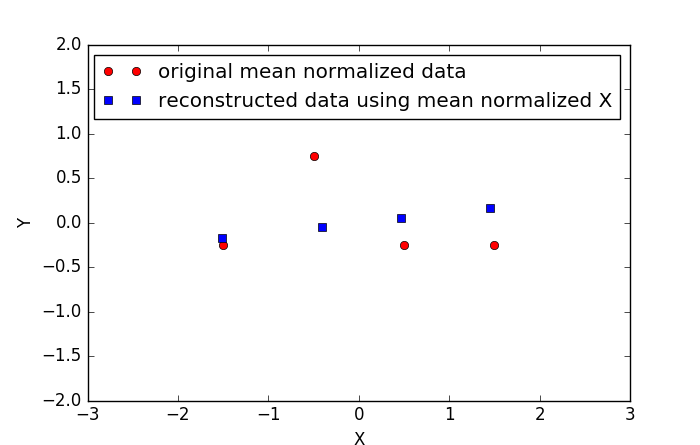
\includegraphics[scale=0.4]{pca_a.png}
	\caption{Plot for part a)}
	\label{fig1}
\end{figure}

Plot for part b):\\
Reconstructed values using the mean-normalized X: $r(x) = g(f(x)) = DD^T x$ \\
\begin{align*}
r(x_1) &\approx (0.17510235, -1.50869279) & r(x_3) &\approx (-0.05393698, 0.46472438)\\ 
r(x_2) &\approx (0.04729127, -0.40746454) & r(x_4) &\approx (-0.16845665, 1.45143296)
\end{align*}

\begin{figure}[ht]
	\centering
	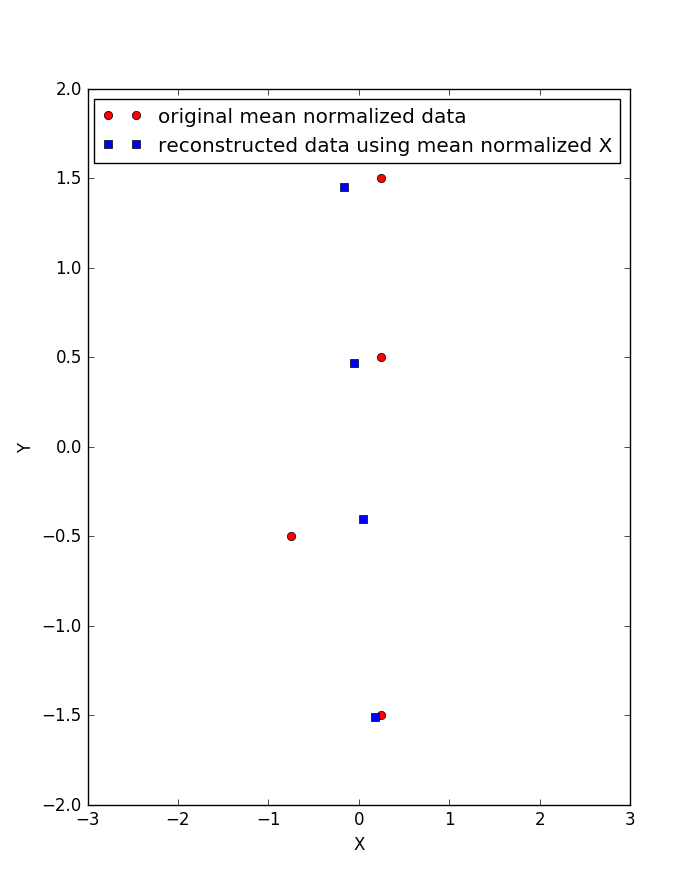
\includegraphics[scale=0.4]{pca_b.png}
	\caption{Plot for part b)}
	\label{fig2}
\end{figure}

\newpage
The red points are original values (normalized), the blue points is the points after reconstructed. We can see from both figures that these blue points lie on a line, because they are reconstructed from a 1-dimension PCA.

\section*{2 Numerical Computation}
\subsubsection*{Ex 2.2}
a)
The idea is to subtract the same value $\lambda$ from all elements of $x_i (i \in [n])$. We will prove that this does not change the value of softmax function:
$$softmax(x_i - \lambda) = \frac{e^{x_i - \lambda}}{\sum\limits_{j=1}^{n}e^{x_j - \lambda}} = \frac{\frac{e^{x_i}}{e^{\lambda}}}{\sum\limits_{j=1}^{n}\frac{e^{x_j}}{e^{\lambda}}} = \frac{\frac{e^{x_i}}{e^{\lambda}}}{\frac{1}{e^{\lambda}} \sum\limits_{j=1}^{n}e^{x_j}} = \frac{e^{x_i}}{\sum\limits_{j=1}^{n}e^{x_j}}\ \ \ \ \ \text{(Hence, proved)}$$

Now we need to choose a value for $\lambda$. The proposed solution is to choose value $\lambda = \max\limits_{j}x_{j}$. After subtracting, the maximum value, the maximum elements in vector \textbf{x} become 0. Hence, the numerator becomes $e^0=1$ for that case, and the denominator $\sum\limits_{j=1}^{n}e^{x_j} > 1$, since there is at least one $e^0 = 1$. This way, we can prevent the overflow. \\
Furthermore, the denominator becoming $\sum\limits_{j=1}^{n}e^{x_j} > 1$ also prevents underflow of the denominator.

Since all entries of x are in the same range of the extreme, the values $x_{i} -\max\limits_{j}x_{j}$ will be close to zero. So, the problem of overflow/underflow may be resolved. 

b)

In case that the range of values in vector \textbf{x} is large (the difference between the largest $x_i$ and smallest $x_j$ is large), the underflow can still happen when evaluating the numerator of softmax function. This will lead to a value of 0 of softmax. Then, if one calculates the log probability of softmax, this will again lead to an underflow value.

\subsubsection*{Ex 2.3}
a) 

See \textbf{gradient\_descent.py}

Final (x,y) = (-0.000000000000, -0.000000000980) $\approx (0, 0)\ |$ f(x,y) = 0.000000000000

b)

\begin{figure}[h]
	\centering
	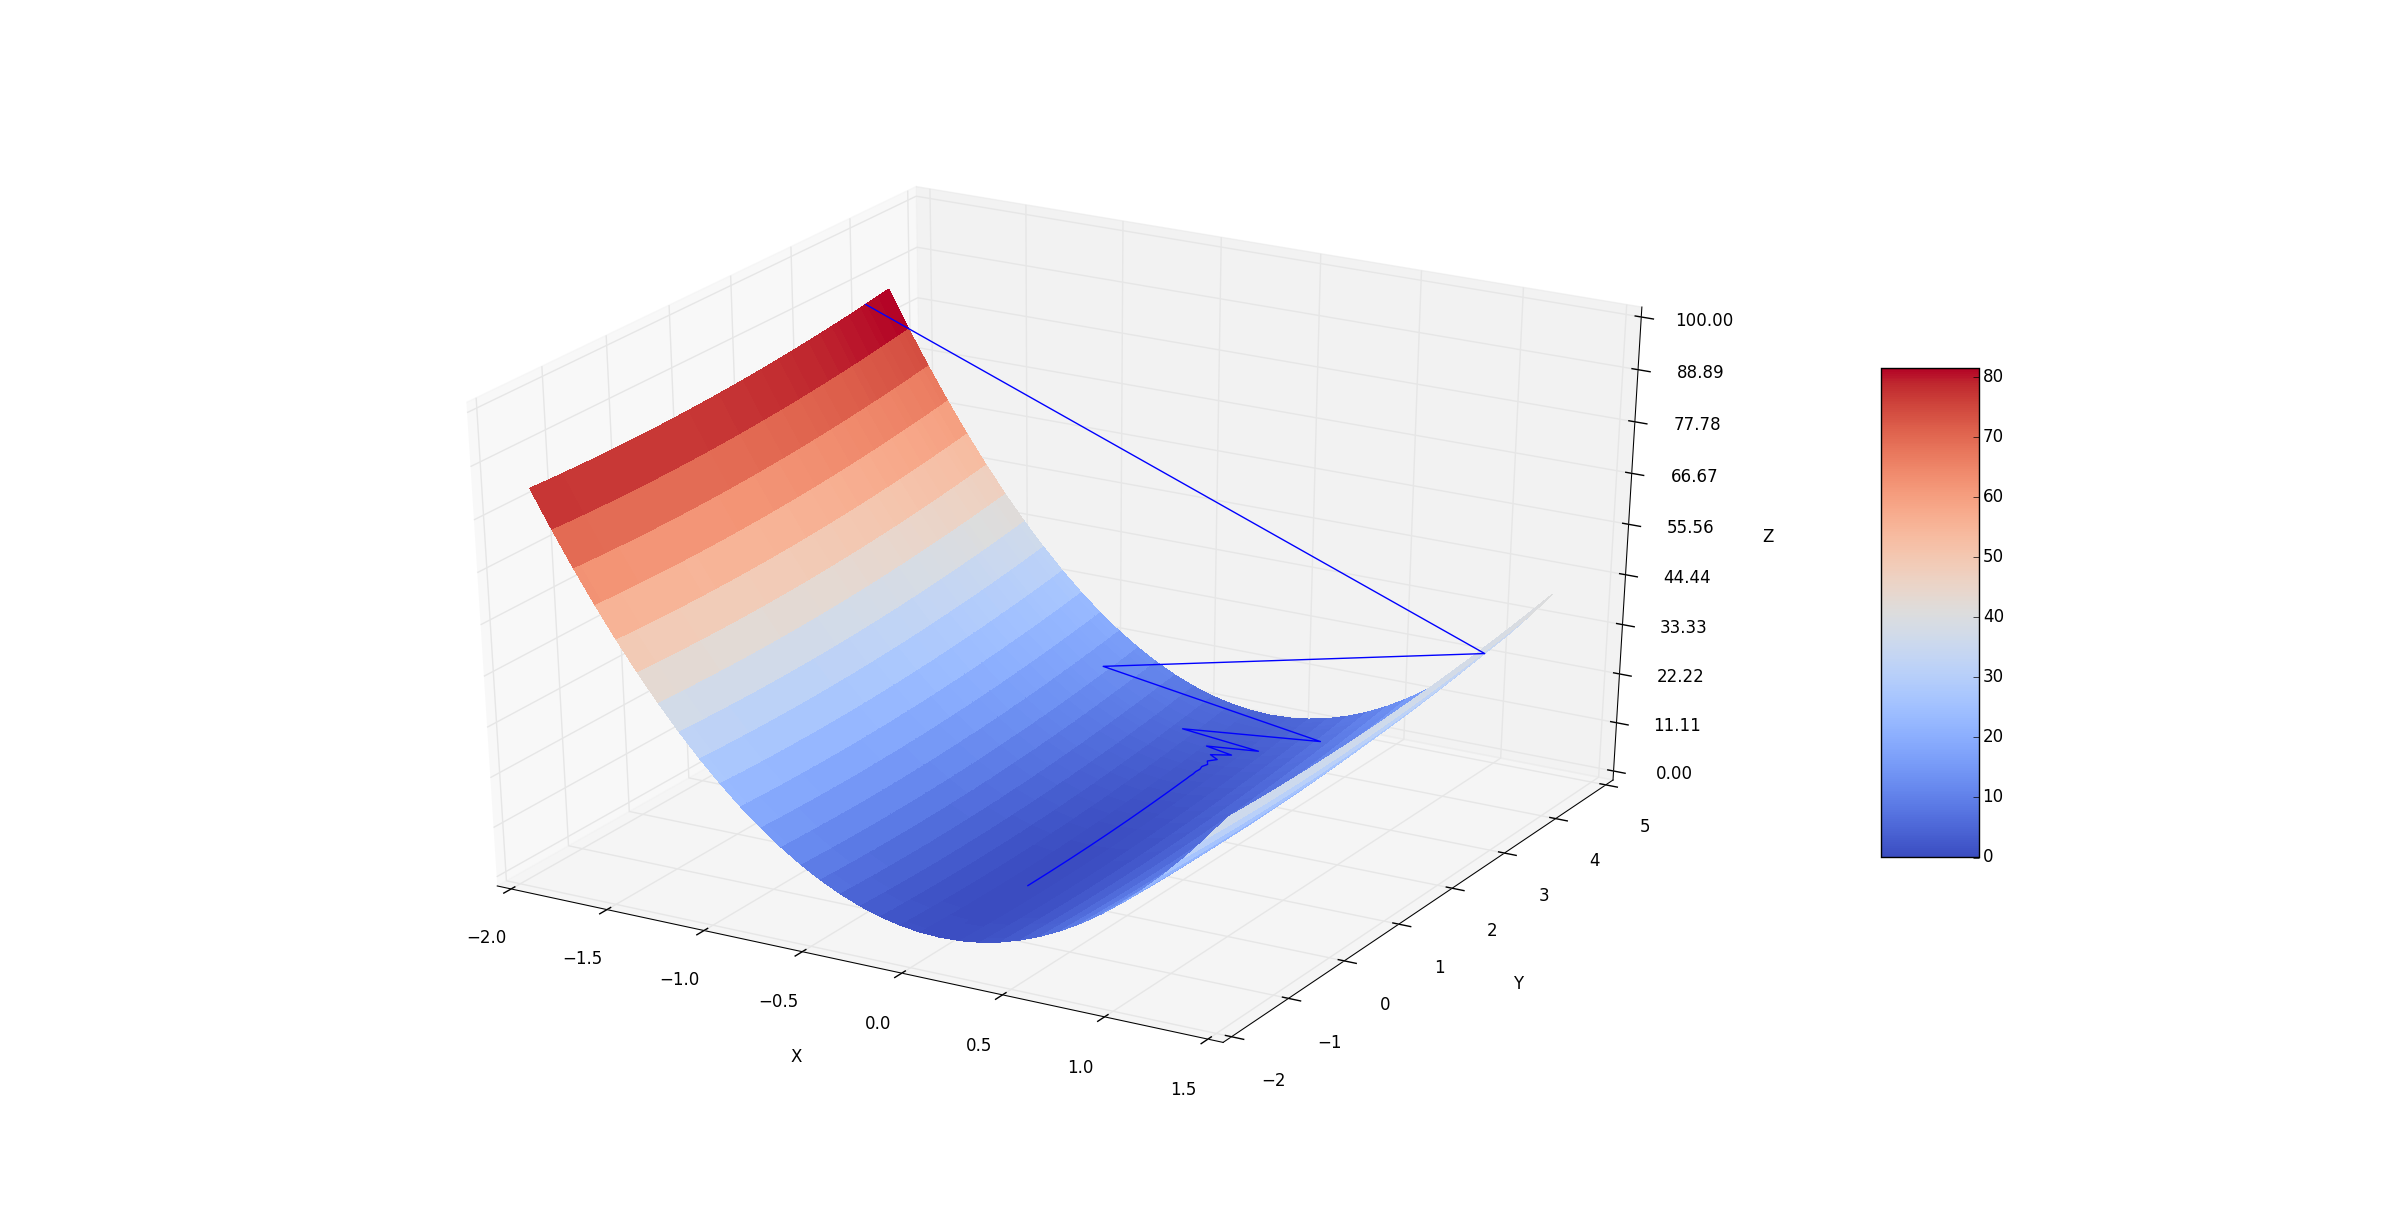
\includegraphics[scale=0.3]{gd.png}
	\caption{Searching with gradient descent}
	\label{fig3}
\end{figure}

Look at Figure \ref{fig3}. At each step, we will calculate the gradient at the current point, which is the partial derivatives of each dimension X and Y at the  current point. If all these derivative values equal to 0, we will stop. Otherwise, we will move the current point with respect to the opposite direction of the gradient, scaled by learning rate. So, after each step, the current point will be closer to the optimal solution. The search path finally reach the optimal solution, which is (0,0).\\
The path looks like a zig-zag line, because the learning rate is quite large but not large enough that the gradient descent algorithm diverges. So it makes quite big steps and sort of ``jumps over'' the optimum value and goes back from there. The zig-zag lines become smaller because the slope becomes smaller when getting closer to the optimum. If the learning rate is too big, however, the steps would overshoot so much that the line then starts to zig-zag uphill, instead of down to the minimum. In this case the gradient descent algorithm diverges.\\
The path shown in Figure \ref{fig3} is not optimal. The optimal path would lead directly to the local minimum.

c)
When changing the learning rate to 0.1, the program will run indefinitely. This is because with a learning rate is too big, at each step, the current point will still continue to move with opposite direction of gradient, but will overshoot through the hill. Hence, it actually will go uphill, which will increase the loss function. It will continue to go uphill without finding the optimal solution. The gradient descent algorithm diverges here.

\newpage

\subsubsection*{Ex 2.4}
a)\\
See \textbf{newton.py}\\
Look at Figure \ref{fig4}
\begin{figure}[h]
	\centering
	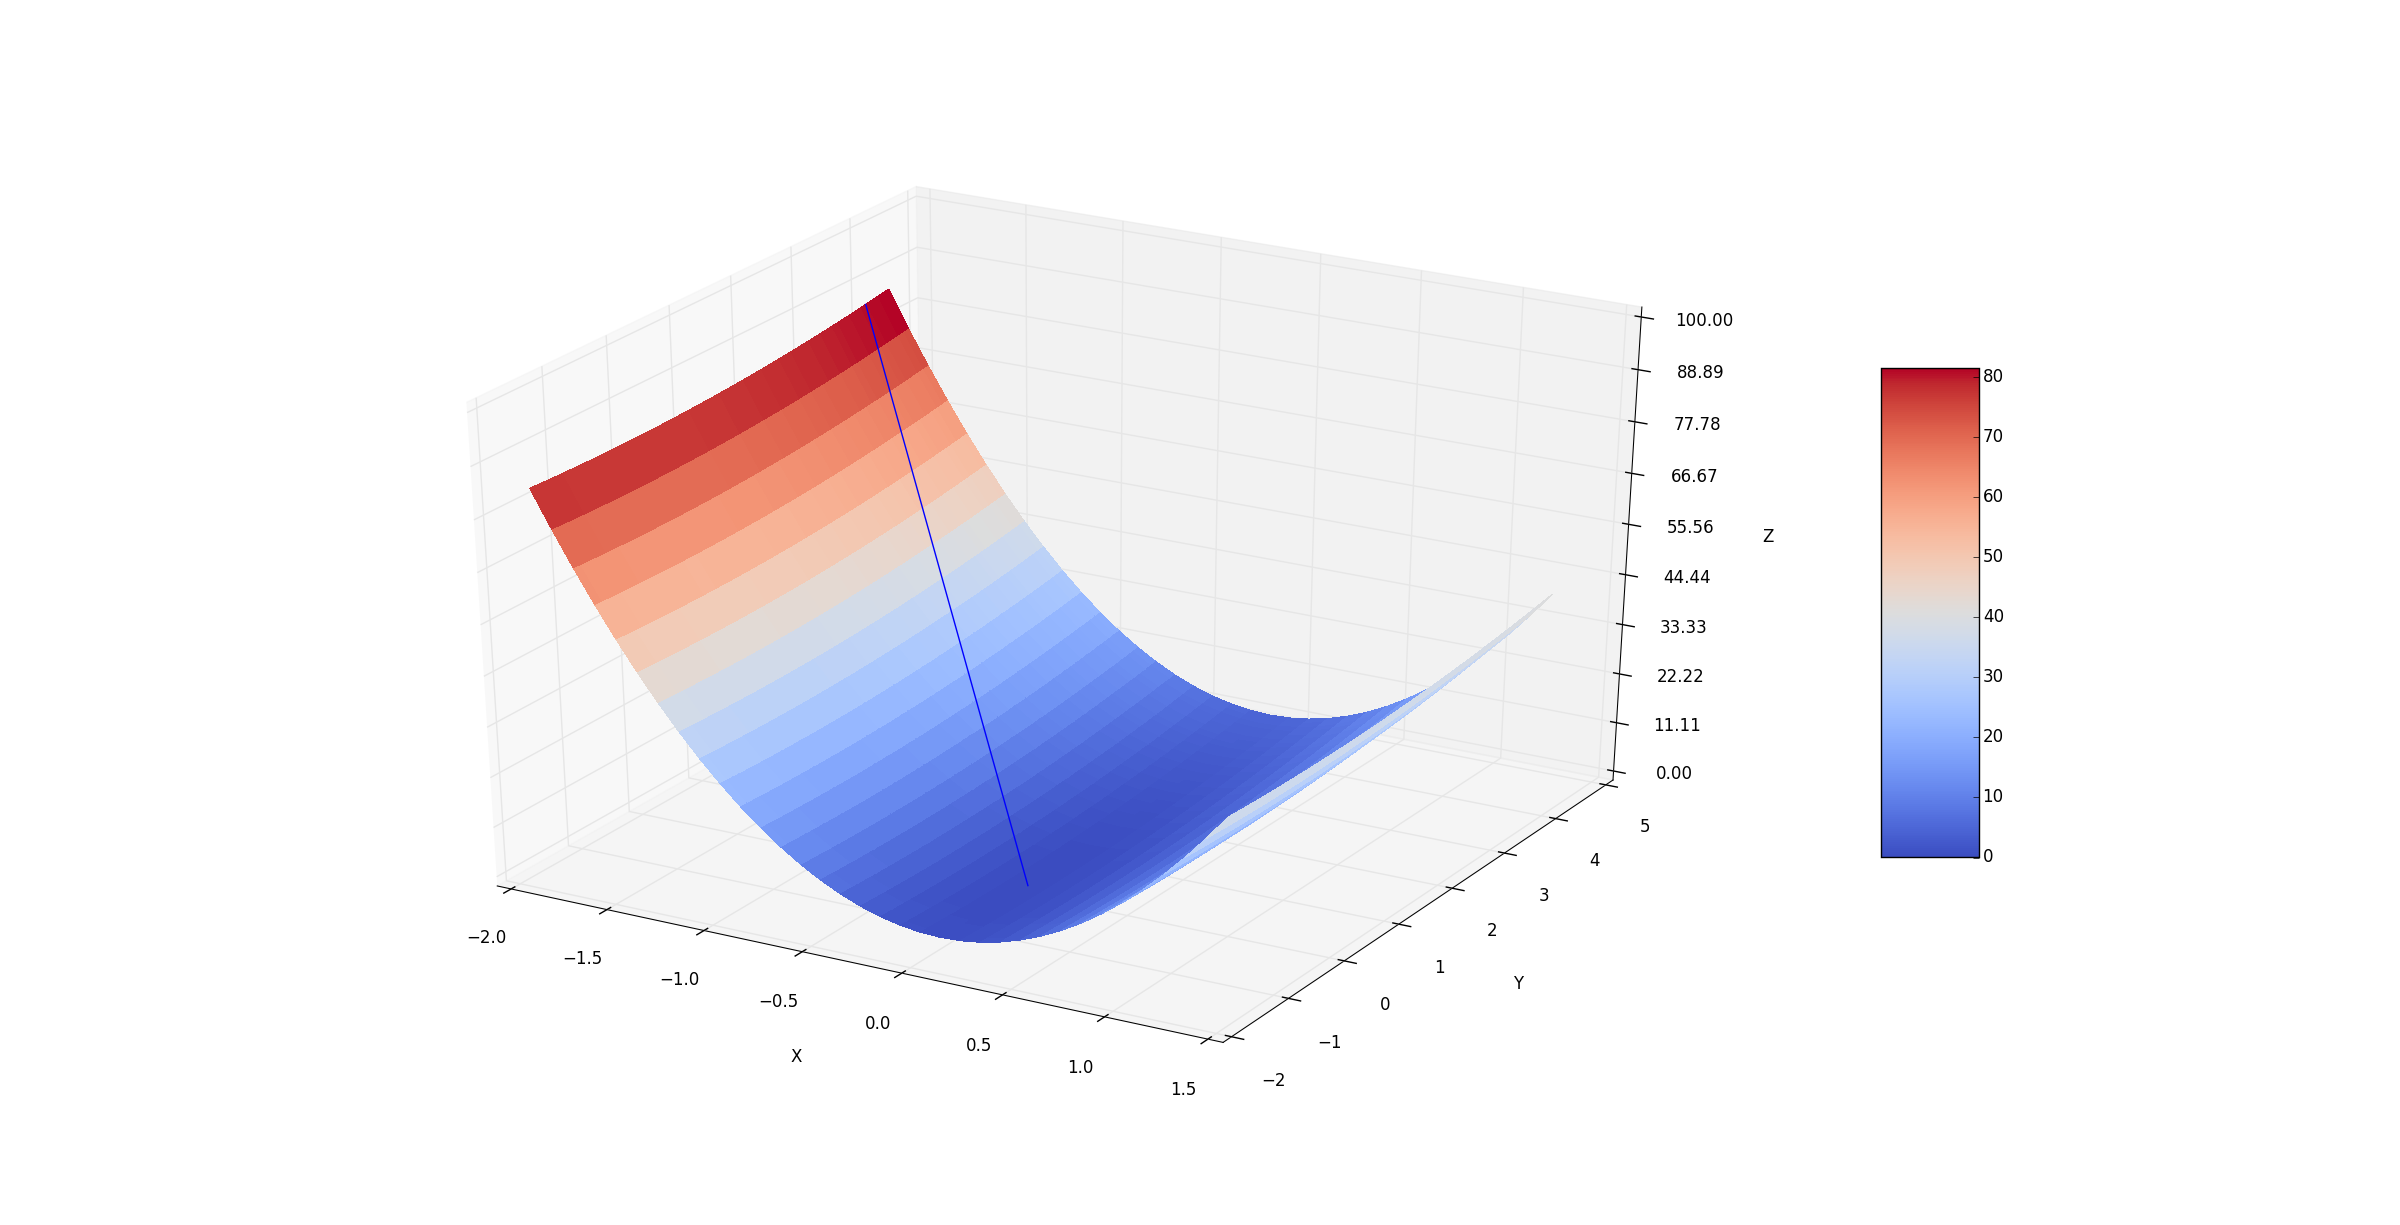
\includegraphics[scale=0.3]{newton.png}
	\caption{Searching with Newton method}
	\label{fig4}
\end{figure}

b)

From Figure \ref{fig4}, we can see that with Newton method, searching is much more faster than gradient descent, because it uses Hessian matrix to guide the search. In this case, the point jump directly to the optimal solution after only one step.

\subsubsection*{Ex 2.5}
A good criterion to stop is we stop when gradient values have absolute value smaller than a threshold (we use the threshold 10$^-9$). Because with very small gradient values, continuing moving does not improve the loss function significantly.
\end{document}



